
\chapter{Markov Decision Processes}

\gls{rl} leverages \glspl{mdp} to model interactions between 
an agent and its environment in terms of states, actions, and rewards. 
This framework captures in a simple way features of the problem such as cause-and-effect, 
uncertainty, and explicit objectives.
Although general \glspl{mdp} may have infinite, possibly uncountable, state and action
spaces, we limit the discussion to finite-state and finite-action problems.

A \gls{mdp} is a model for sequential decision making in a probabilistic environment, it requires
the following components:

\paragraph{States}
The set of environmental states $S$ is defined as the finite set $\{s_1 , . . . , s_N \}$ where the
size of the state space is $|S| = N$. A state is a unique characterization of all
that is important (at given time) of the problem that is modelled. For example, a chess game state 
could be the position of all the pieces on the board.

\paragraph{Actions}
The set of actions A is defined as the finite set $\{a_1 , . . . , a_K \}$ where the size of the
action space is $|A| = K$. Actions can be used to control the system state.
The set of actions that can be applied in some particular state $s \in S$, is denoted $A(s)$,
where $A(s) \subset A$. In some systems, not all actions can be applied in every state, but in
general we will assume that $A(s) = A$ for all $s \in S$.

\paragraph{Trasition Function}
By applying action $a \in A$ in a state $s \in S$, the system makes a transition from s to a
new state $s' \in S$, based on a probability distribution over the set of possible transitions. 
The transition function $\mathcal{T}$ is defined as 
$$\mathcal{T} : S \times A \times S \rightarrow [0,1]$$ which represents the probability
of ending up in state s' after doing action a in state s is denoted $ \mathcal{T}(s,a,s')$. It is required that 
for all actions a, and all states s and s', $\mathcal{T} (s,a,s') \geq 0$ and for all states s and actions a, 
$$\sum_{s' \in S} \mathcal{T} (s,a,s') = 1$$
such that T defines a proper probability distribution over possible next states. \

The sequential nature of the framework is captured by that of \textit{Markov chain}:
a Markovian Stochastic Process. 
Stochastic Processes araise in many problems from the natural sciences
in which one has to keep track of a value observed at time $t$. The process is Markovian if the result of an action does not
depend on the previous actions and history of visited states, but only depends on the
current state.

Going back to our notation, given a trajectory of the form 
$$s_0, a_0, . . . . , s_t, a_t, s_{t+1}$$
the Markov property is defined as follows:

$$P(s_{t+1} | s_t ,a_t ,s_{t_1} ,a_{t-1} , . . ,s_0,a_0) = P(s_{t+1} | s_t ,a_t ) = \mathcal{T} (s_t ,a_t ,s_{t+1} )$$

The idea of Markovian dynamics is that the current state s gives enough information
to make an optimal decision; it is not important which states and actions preceded s.

\paragraph{Reward Function}
Rewards guide learning by signaling success. A higher reward indicates a more 
desirable outcome. In the chess example, capturing a piece might give a large reward, encouraging the 
agent to repeat the actions that led to that success. The reward function $\mathcal{R}$ is usually defined as:
$$\mathcal{R} : S \times A \times S \rightarrow [0,1]$$
which represents the reward received after transitioning from state $s$ to $s'$ by taking action $a$.
Alternatively, the reward function can be defined as $\mathcal{R} : S \times A \rightarrow \mathbb{R}$, 
where the reward depends only on the current state and action. \\


\ With the above components, we can define a \gls{mdp} as in \Cref{fig:mdp}.

\begin{definition}
A \textit{Markov Decision Process} is a tuple $M = (S, A, \mathcal{T}, \mathcal{R})$ where:
\begin{itemize}
    \setlength\itemsep{0.01em}
    \item $S$ is a finite set of states
    \item $A$ is a finite set of actions
    \item $\mathcal{T}$ is the transition function $\mathcal{T} : S \times A \times S \rightarrow [0,1]$
    \item $\mathcal{R}$ is the reward function $\mathcal{R} : S \times A \times S \rightarrow \mathbb{R}$
\end{itemize}
\end{definition}
The transition and reward functions together define the \emph{Model} of
the \gls{mdp}.

\begin{figure}[H]
    \centering
    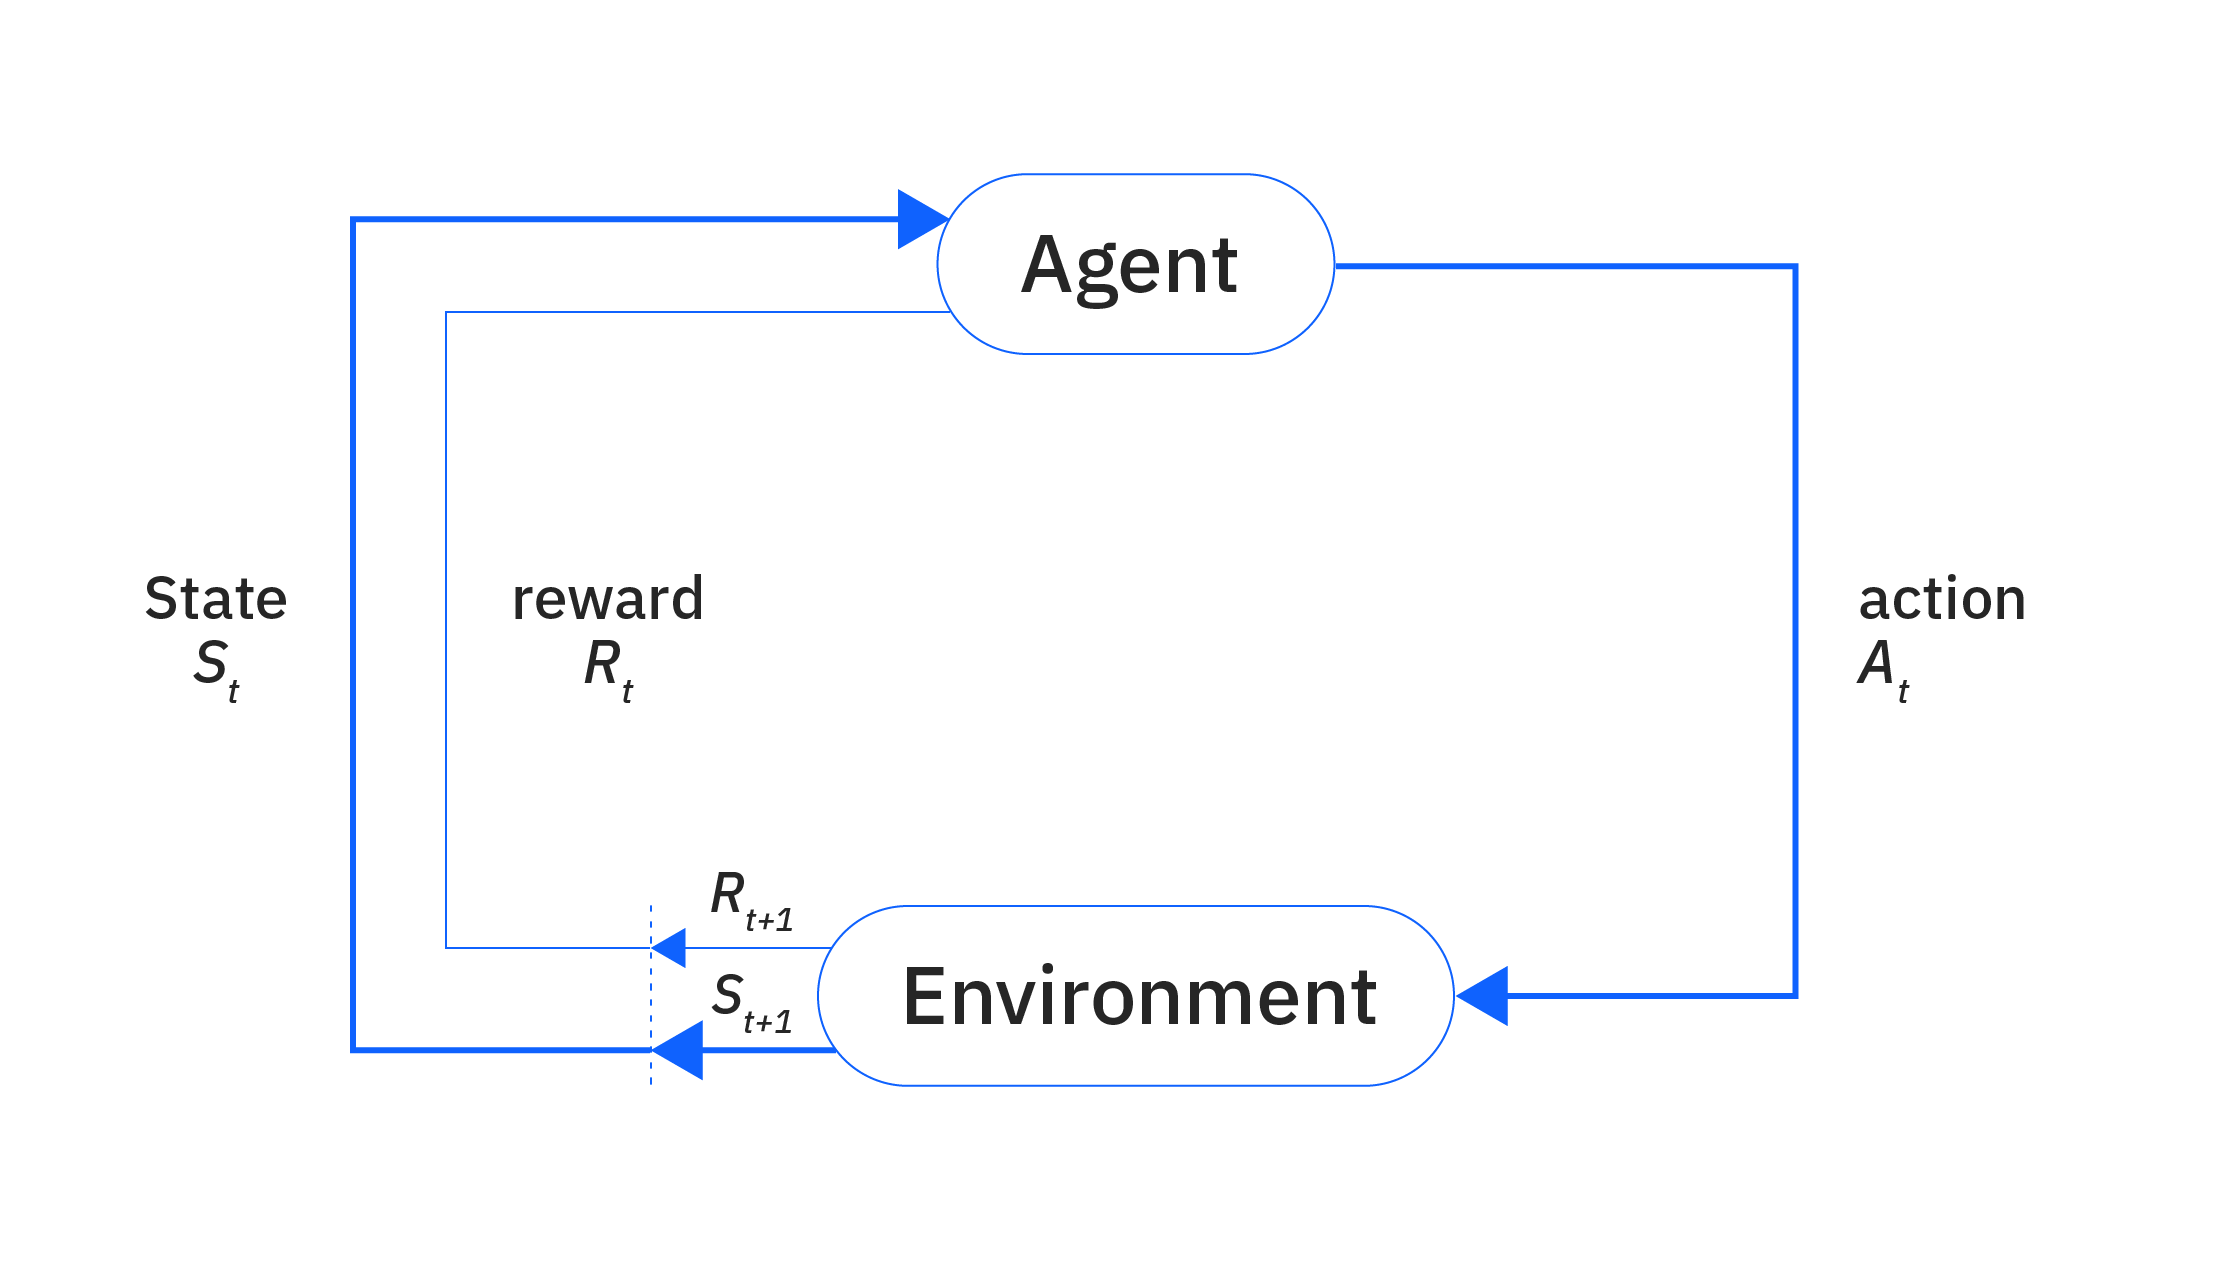
\includegraphics[width=0.5\textwidth]{images/MDP.png}
    \caption{Markov Decision Process}
    \label{fig:mdp}
\end{figure}

A unified notion of transitions and rewards is given by what's called the dynamic of the \gls{mdp}:
$$p : S \times R \times S \times A \rightarrow [0, 1]$$
where
$$p(s' , r |s, a) = Pr\{S_t = s' , R_t = r | S_{t-1} = s, A_{t-1}= a\}$$

$p$ is the probability associated with transitioning from state $s$ choosing action $a$ 
and ending up in state $s'$ and getting reward $r$. Note that the following identities hold:
$$\sum_{s^{\prime} \in S} \sum_{r \in R} p\left(s^{\prime}, r \mid s, a\right)=1 \text {, for all } s \in S, a \in A(s) \text {. }  $$
$$
\mathcal{T}(s,a,s') = p\left(s^{\prime} \mid s, a\right) \doteq \operatorname{Pr}\left\{S_{t}=s^{\prime} \mid S_{t-1}=s, A_{t-1}=a\right\}=\sum_{r \in R} p\left(s^{\prime}, r \mid s, a\right)
$$
and for \(r: S \times A \times S \rightarrow \mathbb{R}\):
$$
\mathcal{R}(s,a,s') = r\left(s, a, s^{\prime}\right) \doteq \mathbb{E}\left[R_{t} \mid S_{t-1}=s, A_{t-1}=a, S_{t}=s^{\prime}\right]=\sum_{r \in \mathcal{R}} r \frac{p\left(s^{\prime}, r \mid s, a\right)}{p\left(s^{\prime} \mid s, a\right)}
$$

These formulations are useful for the analysis of \glspl{mdp} and the development of algorithms. 
In such context, the goal of the agent is to learn an optimal behaviour, let's define behaviours and optimality.

\section{Policy and Value Function}
\paragraph{Policy}
The formalization of the naive concept of behaviour is that of policy. A policy is a function that 
maps states into actions $\pi : S \rightarrow A$. It can be deterministic or stochastic, in 
the latter case it is represented as a probability distribution over actions given states.

$$\pi(a|s) = Pr\{A_t = a | S_t = s\}$$

it holds that for all states $s \in S$, $\pi(a|s) \geq 0$ and $\sum_{a \in A} \pi(a|s) = 1$. 
Another disctinction is made between stationary and nonstationary policies. A stationary policy
does not change over time, it is a function of the current state only,
while a nonstationary policy can be imagined as sequence of policies indexed time. 
In the \emph{finite-horizon} model, a \gls{mdp} in which the agent has a limited amount of time to achieve its goal, 
the optimal policy is typically non stationary: the way an agent chooses its actions on the last step 
of its life is generally going to be very different from the way it chooses them when it has a long
life ahead of it. In the \emph{infinite-horizon} discounted model, the agent always has a constant
expected amount of time remaining, so there is no reason to change action strategies: there
is a stationary optimal policy.   
Such policies represent the strategy of the agent, it is the way the agent interacts with the environment
by iteratively selecting actions based on the current state of the system and thereby influencing the next state and 
reward received. \\
The main goal of \gls{rl} is to find "good" policies. It is intuitive to think that a policy is good 
if it produces high rewards.

% We consider two kinds of policies:
% stationary and nonstationary. A stationary policy, n : S -+ A,is a situation-action mapping
% that specifies, for each state, an action to be taken. The choice of action depends only on the
% state and is independent of the time step. A nonstationary policy is a sequence of situation-
% action mappings, indexed by time. The policy rrt is to be used to choose the action on the
% tth-to-last step as a function of the current state, St. In the finite-horizon model, the optimal
% policy is not typically stationary: the way an agent chooses its actions on the last step of its
% life is generally going to be very different from the way it chooses them when it has a long
% life ahead of it. In the infinite-horizon discounted model, the agent always has a constant
% expected amount of time remaining, so there is no reason to change action strategies: there
% is a stationary optimal policy.   

\paragraph{Value Function} The concept of value function is useful to evaluate the 
quality of a policy. The value function of a state \(s\) under a policy \(\pi\), denoted \(V^{\pi}(s)\), 
is the expected return when starting in \(s\) and following \(\pi\) thereafter. 
We can define the state-value function  \(V^{\pi}\) for policy \(\pi\) in the \emph{discounted infinite model} 
by

$$
V^{\pi}(s) \doteq 
\mathbb{E}_{\pi}\left[\sum_{k=0}^{\infty} \gamma^{k} R_{t+k+1} \mid S_{t}=s \right]
 \text {, for all } s \in S, \quad
$$
% \mathbb{E}_{\pi}\left[G_{t} \mid S_{t}=s\right] 

where \(\mathbb{E}_{\pi}[\cdot]\) denotes the expected value of a random variable given that the agent follows
policy \(\pi\), and \(t\) is any time step, $\gamma \in [0,1]$ is the discount factor, it is used 
to weigh the importance of immediate rewards and to make sure that the sum converges even in 
such infinite horizon problems.
The value function satisfies a recursive relationship known as the \emph{Bellman equation} (\ref{eq:bellman}) 
for \(V^{\pi}\), a crucial concept in the development of learning algorithms.
\begin{align}   
V^{\pi}(s)&=E{\left[\sum_{k} \gamma^k R_{t+k+1}+|S_t=s\right]} \nonumber \\
&=E{\left[G_t|S_t=s\right]} \nonumber \\
&=E{\left[R_{t+1}+\gamma G_{t+1}|S_t=s\right]} \nonumber \\
&= \sum_{s'}\sum_{r}\sum_{g_{t+1}}\sum_{a}p(s',r,g_{t+1}, a|s)(r+\gamma g_{t+1}) \nonumber \\
&= \sum_{a}\pi(a|s)\sum_{s'}\sum_{r}\sum_{g_{t+1}}p(s',r,g_{t+1} |a, s)(r+\gamma g_{t+1}) \nonumber \\
\intertext{since $p(g_{t+1}|s', r, a, s)=p(g_{t+1}|s')$ by MDP assumption}
&= \sum_{a}\pi(a|s)\sum_{s'}\sum_{r}\sum_{g_{t+1}}p(s',r|a, s)p(g_{t+1}|s', r, a, s)(r+\gamma g_{t+1}) \nonumber \\
&= \sum_{a}\pi(a|s)\sum_{s'}\sum_{r}p(s',r|a, s)\sum_{g_{t+1}}p(g_{t+1}|s')(r+\gamma g_{t+1}) \nonumber \\
&= \sum_{a}\pi(a|s)\sum_{s'}\sum_{r}p(s',r|a, s)(r+\gamma\sum_{g_{t+1}}p(g_{t+1}|s')g_{t+1}) \nonumber \\
&=\sum_{a}\pi(a|s)\sum_{s'}\sum_{r}p(s',r|a, s)\left(r+\gamma V^{\pi}(s')\right) \label{eq:bellman}
\end{align}
% notice that p(s',r|s,a) = p(s',r,a|s)p(a|s) allora l'expected value è sum su a s'

Similarly one can define the state-action value function, giving back the value of taking action \(a\) in 
state \(s\) under a policy \(\pi\), denoted
$Q^{\pi}(s, a): S \times A \rightarrow \mathbb{R}$, as the expected return starting from \(s\), taking the action \(a\), and
 following policy \(\pi\) thereafter:
\begin{align}
    Q^{\pi}(s, a) &\doteq \mathbb{E}_{\pi}\left[\sum_{k=0}^{\infty} \gamma^{k} R_{t+k+1} | S_{t}=s, A_{t}=a\right] \nonumber  \\
    &= \mathbb{E}_{\pi}\left[R_t + \gamma V^{\pi}(S_{t+1})| S_{t}=s, A_{t}=a\right] 
\end{align}


it follows naturally that 
\[
    V^{\pi}(s)= \max _{a \in A(s)} Q^{\pi}(s, a)
\]

\section{Bellman Optimality Equation}

Introducing a partial ordering on the space of policies such that 

$\pi \geq \pi' \text{ if and only if } V^{\pi}(s) \geq V^{\pi'}(s) \text{ for all } s \in S$
allows to compare different policies, and to define optimal ones as the class $\pi^*$ 
$$\pi^* \text{ such that } \pi^* \geq \pi \text{ for all } \pi$$

% l'ordine è parziale perchè non è detto che >= valga per ogni s in S ma potrebbe valere solo per alcuni a quel punto non sono confrontabili

\glspl{mdp} (but not \glspl{pomdp}, we'll introduce them in the next chapter), always have\footnote{This 
is true in discrete state space \gls{mdp}s when $\gamma < 1$. 
Existence of optimal policies is not guaranteed in discrete problems for $\gamma = 1$. Generally, in a continous setting, 
it is required $\gamma \in (0,1)$, and costs (negative rewards) to be bounded $|c(s,a)|<M$ for all s and a}
 is a 
deterministic, stationary policy that maximizes the value of every state. \cite{96ef8573-56cc-3a43-a4c7-3c6543c30f4e}
% qualcuno vuole dimostrare l'esistenda stazionarietà e determinismo dell'optimal policy in MDP
    
If we know this optimal policy, then we get the optimal value function $V^{*}(s_{t})$:
\[
V^{*}(s)=\max _{\pi}V^{\pi}(s)
\]
 Similarly, the optimal state-action value function is obtained under the optimal policy:
$$
Q^{*}\left[s_{t}, a_{t}\right]=\max _{\pi} Q^{\pi}\left(s_{t}, a_{t}\right)
$$

Vice versa, knowing the optimal state-action value function allows to derive the optimal policy by 
choosing the action \(a_{t}\) with the highest value
\[
\pi^*\left(s_{t}\right) = \underset{a}{\operatorname{argmax}}\left[Q^{*}\left(s_{t}, a\right)\right]
\]

The optimal value function satisfies the \textit{Bellman Optimality Equation}, given by:

\begin{align}
    V^{\ast }(s)&=\max\limits_{a\in A(s)}Q^{\pi _{\ast }}(s,a) \nonumber \\ 
    & =\max\limits_{a}\mathbb{E}_{\pi _{\ast }}[G_{t}\mid S_{t}=s,A_{t}=a] \nonumber \\ 
    & =\max\limits_{a}\mathbb{E}_{\pi _{\ast }}[R_{t+1}+\gamma G_{t+1}\mid
    S_{t}=s,A_{t}=a] \nonumber \\ 
    & =\max\limits_{a}\mathbb{E}[R_{t+1}+\gamma V^{\ast }(S_{t+1})\mid
    S_{t}=s,A_{t}=a] \nonumber \\ 
    & =\max\limits_{a}\sum\limits_{s^{\prime },r}p(s^{\prime
    },r\mid s,a)\left[ r+\gamma V^{\ast }(s^{\prime })\right].%
    \label{Bellman-optimality-eq}
\end{align}

An analogous result holds for the optimal state-action value function:
\begin{align}
    Q^{\ast }(s,a)&=\mathbb{E}[R_{t+1}+\gamma\max\limits_{a^{\prime }}Q^{\ast
    }(S_{t+1},A_{t+1})\mid S_{t}=s,A_{t}=a] \nonumber \\ 
    & =\sum\limits_{s^{\prime },r}p(s^{\prime },r\mid s,a)\left[ r+\gamma\max\limits_{a^{\prime }}Q^{\ast }(s^{\prime },a^{\prime })\right]. \\
    & = \sum_{s^{\prime}, r} p(s^{\prime}, r | s, a) \left[ r + \gamma V^*(s') \right]
    \label{eq:bellman-state-action}
\end{align}


These equations must be satisfied and can, in principle, be solved for the optimal
value functions, from which an optimal policy can be determined with relative ease.
In practice this is hardly the case due to computational limitations and the optimal value functions 
are usually approximated.

\section{Solving MDPs}
Solving a given \gls{mdp} means computing an optimal policy. The most crucial distinction in available techniques 
is that between \emph{model-based} and \emph{model-free} algorithms. 
Model-based methods use the \gls{mdp} structure explicitly and find the best policy from the transition and reward functions.
If these are known, this is a straightforward optimization problem that can be tackled using dynamic programming. 
If they are unknown, they must first be estimated from observed trajectories.
The main advantage to having a model is that it allows the agent to plan, 
seeing beforehand what would happen in every possible trajectory, and then choosing the best strategy. 
A particularly famous example of this approach is AlphaZero by \cite{Silver2017}.
The presence of a model can result in a substantial improvement in sample efficiency over methods that don't 
exploit it.

The main downside is that a ground-truth model of the environment is usually not available to the agent. 
If an agent wants to use a model in this case, it has to learn the model purely from experience, which 
creates several challenges.


Before diving into modern solution methods - based on \gls{drl} (\cref{fig:drl-algorithm-evolution}) 
and relying on Neural Networks to approximate the value function, the policy, or both - 
we will introduce some of the most common and foundational algorithms used to solve \glspl{mdp} 
that are the building blocks of more advanced techniques.

\begin{figure}
    \centering
    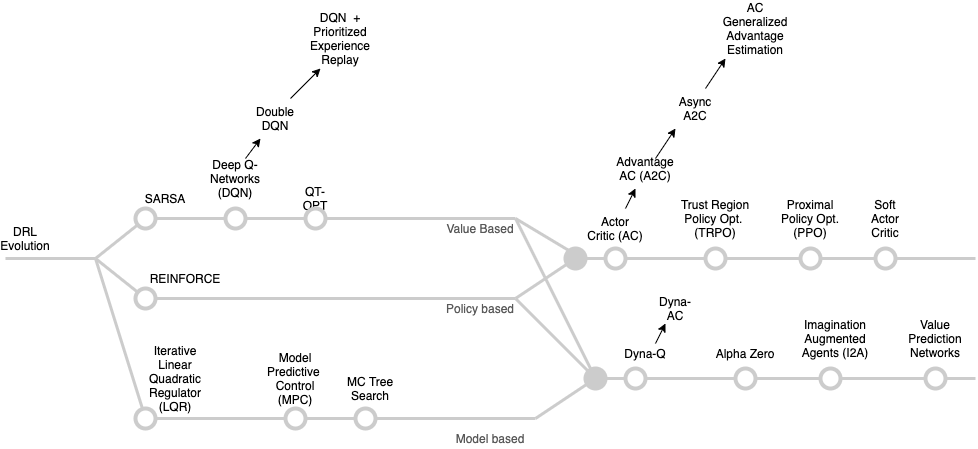
\includegraphics[scale=.35]{images/drl-algorithm-evolution.png}
    \caption{Evolution of Deep Reinforcement Learning Algorithms}
    \label{fig:drl-algorithm-evolution}
\end{figure}

\section{Dynamic Programming}
Dynamic Programming (DP) is a class of algoritms of little practical use, nontheless of great theoretical 
importance in the field of model-based \gls{rl}. The assumption of the availability of the model is 
crucial for the application of these methods as the finitenees of the state and action spaces, though 
continous spaces can be discretized, exact solutions can be rarely found. 
Most \gls{rl} methods work in two main steps: policy evaluation and policy improvement.

\paragraph{Policy Evaluation} policy evaluation or prediction is the task of determining 
the value function for a given policy. If the environment's dynamics are known, \cref{eq:bellman} represents 
a linear system in the $|S|$ unknowns $V^{\pi}(s)$. It can be solved exactly but 
the computational burden of exact solutions, makes iterative methods preferred. 
The most famous of these, known as \textit{Iterative Policy Evaluation}, is based on the Bellman Equation:

$$V^{k+1}(s) = \sum_{a}\pi(a|s)\sum_{s'}\sum_{r}p(s',r|a, s)(r+\gamma V^{k}(s'))$$

where $V^{k}(s)$ is the value function at iteration $k$. The algorithm is guaranteed to converge to the 
true value function $V^{\pi}$ as $k \rightarrow \infty$ under the assumption that $\gamma < 1$ as a 
consequence of the contraction property of the Bellman operator. See \Cref{th:value-iteration} for 
a similar argument proof.

\paragraph{Policy Improvement} 
The purpose of calculating the value function for a policy is to identify better policies. 
To determine if a policy can be improved, we 
compare the value of taking a different action \( a \) in state \( s \) with the current policy. 
This is done using the state-action value function \( Q^\pi(s, a) \):
If $Q^\pi(s, a) > V^\pi(s)$, choosing action $a$ in $s$ is more advantageous than following $\pi$, 
leading to an improved policy $\pi'$. 
\begin{align}
    \pi'(s) & \doteq arg\max_a Q^\pi(s,a) \nonumber\\
    &=  \mathbb{E}[R_{t+1}+\gamma V^{\pi}(S_{t+1})\mid S_t=s,A_t=a] \nonumber\\
    &= arg\max _a \sum_{s', r} p(s',r\,|s,a)\Big[r+\gamma V^{\pi}(s')\Big] \nonumber\\
    \label{eq:policy-improvement}
\end{align}

This is motivated by the following theorem:
\begin{theorem}
    (Policy Improvement Theorem) Let $\pi$ and $\pi'$ be any pair of deterministic policies such that, 
    for all $s \in S$ 
    $$Q^\pi(s, \pi'(s)) \geq V^\pi(s)$$
    Then the policy $\pi' \geq \pi$. That is, it must obtain greater 
    or equal expected return from all states $s \in S$:
    $$V^{\pi'}(s) \geq V^\pi(s)$$
    If there is strict inequality at any state, $\pi'$ is superior to $\pi$.
    \label{th:policy-improvement}
\end{theorem}
\begin{proof}
    \begin{align}
        V^{\pi}(s) &\leq Q^{\pi}(s, \pi'(s)) \nonumber \\
        &= \mathbb{E}\left[R_{t+1} + \gamma V^{\pi}(S_{t+1}) | S_t = s\right] \nonumber \\
        &\leq \mathbb{E}\left[R_{t+1} +\gamma Q^{\pi}(S_{t+1}, \pi'(S_{t+1})) | S_t = s\right] \nonumber \\
        &= \mathbb{E}\left[R_{t+1} + \gamma R_{t+2} + \gamma ^2 V^{\pi}(S_{t+1}) | S_t = s\right] \nonumber \\
        &\leq \dots \nonumber \\
        &=V^{\pi'}(s) \nonumber
    \end{align}
\end{proof}

% \begin{align}
% \pi'(s) &\equiv \arg\max_a Q^\pi(s, a) \nonumber\\
% &= \arg\max_a \mathbb{E}[\mathcal{R}_{t+1} + \gamma V^\pi(\mathcal{S}_{t+1}) \mid \mathcal{S}_t = s, \mathcal{A}_t = a] \nonumber\\
% &= \arg\max_a \sum_{s', r} p(s', r \mid s, a) [r + \gamma V^\pi(s')]  \nonumber
% \end{align}

Policy improvement creates a new policy that enhances an initial policy by adopting a greedy approach 
based on the value function.

\subsection{Policy Iteration}
Policy Iteration allows to estimate an optimal policy in finite time. It is the combination of Policy 
Evaluation and Policy Improvement: once a policy $\pi_t$, has been improved using $V_{t-1}$ to yield 
a better policy $\pi_{t+1}$, we can then compute $V_{t+1}$ and start again. 
\[
\quad \pi_0 \stackrel{\rm E}{\longrightarrow} v_{\pi_0} \stackrel{\rm I}{\longrightarrow} \pi_1 \stackrel{\rm E}{\longrightarrow} v_{\pi_1} \stackrel{\rm I}{\longrightarrow} \pi_2 \stackrel{\rm E}{\longrightarrow} \cdots \stackrel{\rm I}{\longrightarrow} \pi_* \stackrel{\rm E}{\longrightarrow} v_*, \quad
\]
By previous results we can thus obtain a sequence of monotonically improving policies and value functions 
unless we reach the optimal policy.
To show convergence to the optimal policy, along with monotone
improvement, we need to show that if there is no improvement in the value function at any state, then we
are at optimality. Consider k such that 
$V^{\pi_{k+1}} (s) = V^{\pi_{k}}(s), \forall s \in S$. 
We can show using \cref{eq:policy-improvement} that such $V^{\pi_{k}}$ satisfies the Bellman Optimality equation 
\ref{Bellman-optimality-eq}, and hence $V^{\pi_{k}} = V^*$.

The algorithm is summarized in \ref{alg:policy-iteration}.



\begin{algorithm}[H]
    \caption{Policy Iteration}\label{alg:policy-iteration}
    \begin{algorithmic}
    \Require A finite \gls{mdp} with states $S$, actions $A$, transition probabilities $T$, rewards $R$, and discount factor $\gamma \in [0,1]$
    \Ensure Optimal policy $\pi^*$
    \State Initialize an arbitrary policy $\pi$
    \Repeat
        \State \textbf{Policy Evaluation:} Compute the state-value function $V^\pi$
        \State Solve $V^\pi(s) = \sum_{a \in A} \pi(a|s) \sum_{s' \in S} \mathcal{T}(s' | s, a) \left[ \mathcal{R}(s, a, s') + \gamma V^\pi(s') \right]$ for all $s \in S$
        \State \textbf{Policy Improvement:} Compute a new policy $\pi'$
        \ForAll{$s \in S$}
            \State $\pi'(s) \gets \arg\max_{a \in A} \sum_{s' \in S} \mathcal{T}(s' | s, a) \left[ \mathcal{R}(s, a, s') + \gamma V^\pi(s') \right]$
        \EndFor
    \Until{$\pi' = \pi$}  \Comment{Stop when policy converges}
    \State \Return $\pi^*$
    \end{algorithmic}
\end{algorithm}

\subsection{Value Iteration}
The main drawback of Policy Iteration is the need to perform the time consuming policy 
evaluation step at each iteration.
Value Iteration is a simpler alternative that works by truncating the policy evaluation step 
without loosing convergence guarantees, truncating it after a single sweep, results in the following update rule for the 
value function:
\[
\begin{array}{lll}
V_{k+1}(s) & = & \displaystyle \max_{a} \mathbb{E}[R_{t+1}+\gamma V_k(S_{t+1}) \mid S_t=s, A_t=a] \\ 
& = & \displaystyle \max_{a} \sum\limits_{s',r} p(s',r \mid s, a) \left[r+\gamma V_k(s')\right],
\end{array}
\]

or in the equivalent form $V_{t+1} = BV_t$
where $B$ is the \emph{Bellman Optimality Operator} defined as: 
\begin{equation}
    (B^*V)(s) = \max_{a} \sum_{s',r} p(s',r|s,a) \left[ r + \gamma V(s') \right]
    \label{eq:bellman-operator}
\end{equation}
The foundamental theoretical result is that the sequence of value functions $\{V_k\}$ converges to the optimal
value function $V^*$ as $k \rightarrow \infty$.

\begin{lemma}
    The Bellman Optimality operator $B^*$ is a contraction mapping with respect to the
    supremum norm.
    \label{lemma:contraction}
\end{lemma}
\begin{proof}
    Let $V, W$ be any two value functions. Then, for all $s \in S$:
    \begin{align*}
        |(B^*V)(s) - (B^*W)(s)| &= \left| \max_{a} \sum_{s',r} p(s',r|s,a) \left[ r + \gamma V(s') \right] - \max_{a} \sum_{s',r} p(s',r|s,a) \left[ r + \gamma W(s') \right] \right| \\
        &\leq \max_{a} \left| \sum_{s',r} p(s',r|s,a) \left[ r + \gamma V(s') \right] - \sum_{s',r} p(s',r|s,a) \left[ r + \gamma W(s') \right] \right| \\
        &\leq \max_{a} \sum_{s',r} p(s',r|s,a) \left| \left[ r + \gamma V(s') \right] - \left[ r + \gamma W(s') \right] \right| \\
        &\leq \max_{a} \sum_{s'} p(s'|s,a) \left| \gamma V(s') - \gamma W(s') \right| \\
        &\leq \gamma \max_{a} \sum_{s'} p(s'|s,a) \left| V(s') - W(s') \right| \\
        &\leq \gamma \max_{a} \left\| V - W \right\|_{\infty}
    \end{align*}
    where $\left\| V - W \right\|_{\infty} = \max_{s \in S} |V(s) - W(s)|$ is the supremum norm.
\end{proof}

\begin{theorem}
    (Value Iteration Convergence) The sequence of value functions $\{V_k\}$ generated by the value iteration 
    algorithm converges to the optimal value function $V^*$ as $k \rightarrow \infty$.
    \label{th:value-iteration}
\end{theorem}
\begin{proof}
    The result is direct consequence of the contraction property of the Bellman Optimality operator 
    and the Banach Fixed-Point Theorem.
    \begin{align*}
        \left\| V_{k+1} - V^* \right\|_{\infty} &= \left\| B^*V_k - B^*V^* \right\|_{\infty} \\
        &\leq \gamma \left\| V_k - V^* \right\|_{\infty}
    \end{align*}
    By induction, we have that $\left\| V_k - V^* \right\|_{\infty} \leq \gamma^k \left\| V_0 - V^* \right\|_{\infty}$.
    Since $\gamma \in [0,1)$, the sequence $\{V_k\}$ converges to $V^*$.

\end{proof}
The algorithm is summarized in \ref{alg:value_iteration}.

\begin{algorithm}[H]
    \caption{Value Iteration}\label{alg:value_iteration}
    \begin{algorithmic}
    \Require A finite \gls{mdp} with states $S$, actions $A$, transition probabilities $T$, rewards $R$, discount factor $\gamma \in [0,1]$, and a small threshold $\theta > 0$
    \Ensure Optimal policy $\pi^*$
    \State Initialize value function $V(s) \gets 0$ for all $s \in S$
    \Repeat
        \State $\Delta \gets 0$
        \ForAll{$s \in S$}
            \State $v \gets V(s)$
            \State $V(s) \gets \max_{a \in A} \sum_{s' \in S} \mathcal{T}(s, a,s') \left[ \mathcal{R}(s, a, s') + \gamma V(s') \right]$
            \State $\Delta \gets \max(\Delta, |v - V(s)|)$
        \EndFor
    \Until{$\Delta < \theta$}  \Comment{Stop when value function converges}
    \State \textbf{Extract Policy:}
    \ForAll{$s \in S$}
        \State $\pi^*(s) \gets \arg\max_{a \in A} \sum_{s' \in S} \mathcal{T}(s,a,s') \left[ \mathcal{R}(s, a, s') + \gamma V(s') \right]$
    \EndFor
    \State \Return $\pi^*$
    \end{algorithmic}
\end{algorithm}

\subsection{Generalized Policy Iteration}
A very important underlying mechanism, common to most methods, is the so-called \gls{gpi} principle. 
It consists of two interacting processes. 

First the policy evaluation step estimates the utility
of the current policy, computing $V^{\pi}$, directly through the use of the model (if available)
or iteratively by sampling trajectories interacting with the environment.
Second the policy improvement step computes an improved policy from the current one using the information in $V$. 

Both the evaluation and the improvement steps can be implemented and interleaved in several distinct ways. 
The underliyng mechanism is that there is a policy that drives value learning, i.e. it determines the value function, but in
turn there is a value function that can be used by the policy to select good actions.

\begin{figure}
    \centering
    \includegraphics[scale=.2]{images/gpi.png}
    \caption{Generalized Policy Iteration}
    \label{fig:gpi}
\end{figure}

\section{Monte Carlo Methods}
Learning methods do not necessarly need to rely on the model of the environment. Model free techniques 
are based on the idea of learning from actual or simulated\footnote{Although a model is 
needed for simulated experience, a sample model is sufficient and is way easier to obtain than a 
full probabilistic specification of the environment dynamics} experience, in the form of sample sequence of states, 
actions and rewards.
Following the \gls{gpi} framework we briefly explore the main ideas behind \gls{mc} Methods.

\paragraph{Policy Evaluation} The most intuitive strtegy for estimating the value function without a model 
is to average rewards after visiting a state.
In particular, if we had to estimate $V_{\pi}(s)$, given a set of episodes obtained by following ${\pi}$
after s, since s may be visited multiple times in the same episode; denoting the first time it is 
visited in an episode the \textit{first visit} to $s$, two options are available:
\begin{itemize}
    \item First-visit \gls{mc} method estimates V(s) as the average of the returns following first visits to s.
    \item Every-visit \gls{mc} method averages the returns following all visits to s.
\end{itemize}

Convergence of both methods is guaranteed by the law of large numbers.

\paragraph{Policy improvement}
It is worth noting that the absence of the model, state values alone are not sufficient to determine a 
greedy policy w.r.t. $V$. For control tasks \gls{mc} methods are therefore used to estimate the action-value function
$Q^{\pi} (s, a)$. 
The concept of visits is redefined to apply to state-action pairs, rather than states alone: a 
state-action pair $(s, a)$ is considered visited if action $a$ was selected while in state $s$

\paragraph{Monte Carlo Control}
In policy evaluation, we need to be cautious and ensure that all
states will be visited, otherwise convergence is not guaranteed. To accomplish this we can generate the 
episodes with \textit{exploring starts}, that is, all episodes begin with state-action pairs randomly
selected to cover all possibilities.
The second underlying assumption we made is that policy evaluation could be done over an infinite number of 
episodes. Under theses assumptions, the value function converges to the true value function by 
\textit{Policy Improvement Theorem} \ref{th:policy-improvement}. 

Both assumptions can actually be relaxed by giving up on deterministic policies, only search over
$\epsilon$-soft policies \ref{eq:epsilon-soft}, and by allowing the value function to be updated after each episode and 
not when convergence is met.

\begin{equation}
    \pi(a|s)=\left\{
    \begin{array}{ll}
    1-\epsilon+\frac{\epsilon}{|A|} & \mbox{if $a=\mbox{argmax}_{a'}Q^{\pi}(s,a')$} \\
    \frac{\epsilon}{|A|} & \mbox{otherwise}
    \end{array}
    \right.
    \label{eq:epsilon-soft}
\end{equation}


\begin{algorithm}
    \caption{Monte Carlo Control with Exploring Starts}\label{alg:monte_carlo}
    \begin{algorithmic}
    \Require A finite \gls{mdp} with states $S$, actions $A$, rewards $R$, discount factor $\gamma \in [0,1]$, and an exploring-starts assumption
    \Ensure Optimal policy $\pi^*$
    
    \State Initialize arbitrary action-value function $Q(s, a)$ for all $s \in S$, $a \in A$
    \State Initialize returns list $\text{Returns}(s, a) \gets \emptyset$ for all $s, a$
    \State Initialize policy $\pi$ arbitrarily
    \Repeat
        \State Generate an episode: $(s_0, a_0, r_1, s_1, a_1, r_2, \dots, s_T)$ following $\pi$
        \State $G \gets 0$
        \For{$t = T-1$ to $0$}  \Comment{Process the episode in reverse}
            \State $G \gets \gamma G + r_{t+1}$
            \If{$(s_t, a_t)$ is the first occurrence in the episode}
                \State Append $G$ to $\text{Returns}(s_t, a_t)$
                \State $Q(s_t, a_t) \gets \frac{1}{|\text{Returns}(s_t, a_t)|} \sum \text{Returns}(s_t, a_t)$
                \State Update policy: $\pi(s_t) \gets \arg\max_{a \in A} Q(s_t, a)$
            \EndIf
        \EndFor
    \Until{Q-values converge}
    
    \State \Return $\pi^*$
    \end{algorithmic}
\end{algorithm}

\section{Temporal Difference Learning}
Combining the ideas of \gls{dp} and \gls{mc} methods, \gls{td} learning is a model-free method that 
learns from experience (like \gls{mc}) but updates estimates based on other learned estimates 
(like \gls{dp}), a technique known as bootstrapping.

\gls{td} prediction methods update the value function estimates based on the difference between the
current estimate and a target value, which is a sum of the reward and the value of the next state.
The simplest form of \gls{td} prediction is the \gls{td}(0) algorithm, also known as the one-step \gls{td}
algorithm. The update rule for the value function is given by:
\[
V(S_t) \leftarrow V(S_t) + \alpha \Big[ R_{t+1} + \gamma V(S_{t+1}) - V(S_t) \Big]
\]
Convergence results for TD(0) is found in \cite{10.1023/A:1022633531479}, For any fixed policy $\pi$, 
TD(0) has
been proved to converge to $V_\pi$, in the mean for a constant step-size parameter if it is
sufficiently small, and with probability 1 if the step-size parameter decreases according to
the usual stochastic approximation conditions:
\begin{equation}
\sum_{n=1}^{\infty}\alpha_{n}(a)=\infty\quad\quad\quad\mbox{and}\quad\quad\sum_{n=1}^{\infty}\alpha_{n}^{2}(a)<\infty.
\end{equation}

We present two \gls{td} control methods that are widely used in practice: Sarsa and Q-Learning.

\subsection{Sarsa} Sarsa is an on-policy method that updates the action-value function Q based on the
current policy $\pi$ and the action taken in the next state. The update rule is given by:
\[
Q(S_t,A_t) \leftarrow Q(S_t,A_t) + \alpha \Big[ R_{t+1} + \gamma Q(S_{t+1},a) - Q(S_t,A_t) \Big].
\]
The convergence properties of the Sarsa algorithm depend on the nature of the policy’s
dependence on Q. For example, one could use $\epsilon$greedy or $\epsilon$-soft policies. Sarsa converges
with probability 1 to an optimal policy and action-value function as long as all state–action
pairs are visited an infinite number of times and the policy converges in the limit to
the greedy policy.

\subsection{Q-Learning}
A similar update for an off-policy method is given by the Q-Learning algorithm by \cite{Watkins1992Qlearning}:
\[
Q(S_t,A_t) \leftarrow Q(S_t,A_t) + \alpha \Big[ R_{t+1} + \gamma \max_a Q(S_{t+1},a) - Q(S_t,A_t) \Big].
\]
In this case, the learned action-value function, $Q$, directly approximates the optimal
action-value function $Q^*$,  independent of the policy being followed. This dramatically
simplifies the analysis of the algorithm and enabled early convergence proofs. The policy
still has a crucial role in that it determines which state-action pairs are visited,
and it is required for convergence that all pairs continue to be updated.

Q-learning is one of the most well known and widely used algorithms in \gls{rl} and has been
extended and adapted in many ways. The convergence of Q-learning has been proved for
many cases, including linear function approximation, and it has been shown to be a very
effective and robust method in practice.

\section{Policy Gradient Methods}
We now consider methods that directly learn the policy, rather than the value function.
Policy gradient methods are a class of algorithms that search for the optimal policy by
updating the policy parameters in the direction that increases the expected return making use of its gradients. 

The first concept we  will present is that of Function Approximation in the context of \gls{rl}, than we'll present the foundamental 
theoretical result of Policy Gradient Methods: the \emph{Policy Gradient Theorem} \ref{pg_theorem}. 
Finally we'll explore some of the most common algorithms based on this principle.  

\subsection{Function Approximation}
Up to now we have considered the case in which the value function or the policy  
are represented exaclly as tables. This is hardly done in practice, as prohibitively large state and action spaces 
require a more compact representation. Function approximation comes in handy as a technique used to store 
function information and generalize to unseen transitions efficiently. The most common function 
approximators are Neural Networks, followed by kernel functions, linear models, decision trees, and others. 
In such cases the value function or the policy are represented by a parameterized function,
$V(s; \theta)$ or $\pi(a|s; \theta)$, where $\theta$ is the parameter vector of the function approximator.
Once the function approximator is defined, the goal is to find the optimal parameters $\theta^*$ that 
maximize the expected return, most of the times by Stochastic Gradient Descent\footnote{\gls{sgd} was first introduced by \cite{10.1214/aoms/1177729586}}.

Consider the problem of finding the value function corresponding to a policy \(\pi\), thus far we 
implemented the update rule for the value function by moving the value prediction $V(s)$ closer to 
the return $G_t$, which represents the target:
$$V(s) = V(s) + \alpha (G_t - V(s))$$

Function approximation allows to perform the same update on the parameter vector $\theta$ as follows:

$$\theta_{t+1} \doteq \theta_t + \alpha (U_t - V(s_t;\theta_t)) \nabla V(s_t;\theta_t)$$

where $U_t$ is the unbiased estimate for the target value $V_\pi$, and $\nabla V(s_t;\theta_t)$ is the gradient of the value function
with respect to the parameter vector $\theta$.



\subsection{Policy Gradient Theorem}\label{sec:pg_theorem}

Now consider a parameterized policy \(\pi_\theta\), which is differentiable almost everywhere, and the following objective function \(J\) for maximizing the expected episodic return: 
\begin{align*}
	J(\theta) &= \mathbb{E}_{S_0 \sim p_0, \pi_\theta} \bigl[ G_0 \bigr] \\
	&= \mathbb{E}_{S_0 \sim p_0} \Bigl[ \mathbb{E}_{\pi_\theta} \bigl[ G_t \mid S_t = S_0 \bigr] \Bigr] \\
	&= \mathbb{E}_{S_0 \sim p_0} \Bigl[ V_{\pi_\theta}(S_0) \Bigr]
\end{align*}

In this section we treat the episodic case, for which we define the performance measure
as the value of the start state of the episode. We can simplify the notation without
losing any meaningful generality by getting rid of the initial state distribution $p_0$ assuming that every episode starts in some particular
(non-random) state $s_0$:
\begin{align*}
    J(\theta) = V^{\pi_{\theta}}(s_0)
\end{align*}

The idea of policy gradient algorithms is to maximize \(J(\theta)\) over the parameters \(\theta\) by performing gradient ascent \cite{Sutton1998}. 
Hence, we require the gradients \(\nabla_\theta J(\theta)\), however it is a priori not obvious how 
the right-hand side \(\mathbb{E}_{S_0 \sim p_0, \pi_\theta} \bigl[ G_0 \bigr]\) depends on \(\theta\) 
as changes in the policy \(\pi\) also affect the state distribution \(d^\pi\). The Policy Gradient 
Theorem \cite{NIPS1999_464d828b, 905687} yields an analytic form of 
\(\nabla_\theta J(\theta)\) from which we can sample gradients that does not involve the derivative 
of \(d^\pi\). Here, we focus on the undiscounted case, i.e. \(\gamma = 1\). Note that any discounted 
problem instance can be reduced to the undiscounted case by letting the reward function absorb the 
discount factor \cite{schulman2018highdimensionalcontinuouscontrolusing}.

\begin{theorem} \label{pg_theorem}
	(Policy Gradient Theorem)
	For a given MDP, let \(\pi_\theta\) be differentiable w.r.t. \(\theta\) and \(\nabla_\theta \pi_\theta\) be bounded, let \(Q^{\pi_\theta}\) be differentiable w.r.t. \(\theta\) and \(\nabla_\theta Q^{\pi_\theta}\) be bounded for all \(s\) and \(a\). Then, there exists a constant \(\eta\) such that
	\begin{equation}
		\nabla_\theta J(\theta) = \eta \: \mathbb{E}_{S \sim d^{\pi_\theta}, A \sim \pi_\theta} \Bigl[ Q^{\pi_\theta}(S,A) \: \nabla_\theta \ln \pi_\theta(A \mid S) \Bigr]. \label{eq:pg_theorem}
	\end{equation}
\end{theorem}
\begin{proof}
	We follow the proof by \cite{Sutton1998} the detailed one by \cite{lehmann2024definitiveguidepolicygradients}.
	To simplify the notation, we omit subscripts \(\theta\) for the policy \(\pi\) and all gradients \(\nabla\) but both always depend on the parameters \(\theta\).
	
	Starting from the definition of the objective function, use the relationship between value and action-value function, 
	\( V^\pi (s) = \sum_{a} \pi(a \mid s) \: Q^\pi (s, a) \: \) 
	and the product rule.
	\begin{align}
		\nabla \: V^\pi(s) \: &= \nabla \sum_{a} \pi(a \mid s) \: Q^\pi(s,a) \: \nonumber \\
		&= \sum_{a} \nabla \pi(a \mid s) \: Q^\pi(s,a) \: + \sum_{a} \pi(a \mid s) \: \nabla Q^\pi(s,a) . \label{eq:pgproof_1}
	\end{align}
	
	Now, consider the recursive formulation of the action-value function 
	\[Q^\pi(s,a) = \sum_{s'} \sum_{r} p(s', r \mid s,a) \: \bigl(r + V^\pi(s')\bigr) .\]
	Due to the identity \(\sum_{r} p(s', r \mid s,a) = p(s' \mid s,a)\) and since realized rewards \(r\) and environment transitions for a given action no longer depend on the policy, we can reformulate the gradients of \(Q^\pi\) w.r.t. \(\theta\).
	\begin{align}
		\nabla Q^\pi(s,a) &= \nabla \sum_{s'} \sum_{r} p(s', r \mid s,a) \: \bigl(r + V^\pi(s')\bigr) \: \nonumber \\
		% exchange differentiation and integration
		&= \sum_{s'} \sum_{r} p(s', r \mid s,a) \: \nabla \bigl(r + V^\pi(s')\bigr) \: \nonumber \\ 
		% r does not depend on \theta
		&= \sum_{s'} \sum_{r} p(s', r \mid s,a) \: \nabla V^\pi(s') \: \nonumber \\ 
		 % using sum over r = omit r
		% &= \nabla \sum_{s'} p(s' \mid s,a) V^\pi(s') \\ 
		% exchange integration and differentiation 
		&= \sum_{s'} p(s' \mid s,a) \: \nabla V^\pi(s') \: \label{eq:pgproof_2}.
	\end{align}
	% Further, note that for all \(s\) as in Equation \eqref{eq:pgproof_1} the following holds:
	% \begin{align}
	% 	\nabla V^\pi(s) &= \sum_{a} \nabla \pi(a \mid s) \: Q^\pi(s,a) + \sum_{a} \pi(a \mid s) \: \nabla Q^\pi(s,a), \label{eq:pgproof_3}
	% \end{align}
	
    By using \eqref{eq:pgproof_1} and \eqref{eq:pgproof_2}, we can transform \eqref{eq:pgproof_1} into a recursive form, which we are then going to unroll subsequently to yield an explicit form. In the following, we simply notation by defining 
	\begin{equation}
		\label{eq:pgproof_4}
		\phi(s) \coloneqq \sum_{a} \nabla \pi(a \mid s) \: Q^\pi(s,a).
	\end{equation}
	Applying \eqref{eq:pgproof_4} and \eqref{eq:pgproof_2} to \eqref{eq:pgproof_1} in order and rearranging the integrals gives
	\begin{align}
		\nabla J(\theta) &=  \: \sum_{a} \nabla \pi(a \mid s) \: Q^\pi(s,a) da + \sum_{a} \pi(a \mid s) \: \nabla Q^\pi(s,a) \:  \nonumber \\
		&=  \: \phi(s) +  \sum_{a} \pi(a \mid s) \: \nabla Q^\pi(s,a) \: ds \nonumber \\
		&=  \: \phi(s) + \sum_{a} \pi(a \mid s) \: \sum_{s'} p(s' \mid s,a) \: \nabla V^\pi(s') \: \:  \nonumber \\
		% Fubini 
		&=  \: \phi(s) + \sum_{s'} \sum_{a} \pi(a \mid s) \: p(s' \mid s,a) \: \nabla V^\pi(s') \: \:  \label{eq:pgproof_5}
	\end{align}
	To unroll Equation \eqref{eq:pgproof_5} across time, we introduce notation for multi-step transition probabilities. Let \(\rho_\pi (s \to s', k)\) be the probability of transitioning from state \(s\) to \(s'\) after \(k\) steps under policy \(\pi\). We have that 
	\[\rho_\pi (s \to s', 0) \coloneqq 
	\begin{cases}
		1 & \text{if } s = s',\\
		0 & \text{else}
	\end{cases}
	\] 	
	and \(\rho_\pi (s \to s', 1) \coloneqq \sum_{a} \pi(a \mid s) \: p(s' \mid s,a)\). 
	Now, we can recursively write
	\[\rho_\pi (s \to s'', k+1) = \sum_{s'} \rho_\pi (s \to s', k) \: \rho_\pi (s' \to s'', 1) \:.\]
	Using this notation, iteratively substituting in \eqref{eq:pgproof_1} and \eqref{eq:pgproof_2}, we can unroll \eqref{eq:pgproof_5}:
	\begin{align*}
		\nabla J(\theta) &=  \: \phi(s) + \sum_{s'} \sum_{a} \pi(a \mid s) \: p(s' \mid s,a) \: \nabla V^\pi(s') \: \:  \\
		&=  \: \phi(s) + \sum_{s'} \rho_\pi (s \to s', 1) \: \nabla V^\pi(s') \: \:  \\
		&=  \: \phi(s) + \sum_{s'} \rho_\pi (s \to s', 1) \: \phi(s') + \sum_{a} \pi(a \mid s') \: \nabla Q^\pi(s',a) \: \:  \\
		&=  \: \phi(s) + \sum_{s'} \rho_\pi (s \to s', 1) \: \phi(s') + \sum_{s''} \rho_\pi (s' \to s'', 1) \: \nabla V^\pi(s'') \:' \: \:  \\ 
		&=  \: \phi(s) + \sum_{s'} \rho_\pi (s \to s', 1) \: \phi(s') \: \\
		&\qquad + \sum_{s''}\sum_{s'} \rho_\pi (s \to s', 1) \: \rho_\pi (s' \to s'', 1) \ \: \nabla V^\pi(s'') \:' \: \:  \\ 
		&=  \: \phi(s) + \sum_{s'} \rho_\pi (s \to s', 1) \: \phi(s') \: + \sum_{s''} \rho_\pi (s \to s'', 2) \: \nabla V^\pi(s'') \:' \:  \\
		&=  \: \rho_\pi (s \to s, 0) \phi(s) + \sum_{s'} \rho_\pi (s \to s', 1) \: \phi(s') \: \\ 
		&\qquad + \sum_{s''} \rho_\pi (s \to s'', 2) \: \phi(s'') \:' + \sum_{s'''} \rho_\pi (s \to s''', 3) \: \nabla V^\pi(s''') \:'' \:  \\
		&\;\;\vdots \\
		&=  \sum_{s'} \sum^T_{t=0} \rho_\pi (s \to s', t) \: \phi(s') \: \: 
	\end{align*}
	We set \(\eta_s(s') \coloneqq \sum^T_{t=0} \rho_\pi (s \to s', t)\) to obtain 
	\begin{align}
		\nabla_\theta J(\theta) &=  \sum_{s'} \sum^T_{t=0} \rho_\pi (s \to s', t) \: \phi(s') \: \:  \nonumber \\
		&= \sum_{s'}  \: \eta_s(s') \: \phi(s') \:  \: \nonumber \\
		&= \frac{\sum_{s''}  \eta_s(s'') \:  \:'}{\sum_{s''}  \eta_s(s'') \:  \:'} \sum_{s'}  \: \eta_s(s') \:  \: \phi(s') \: \nonumber \\
		&= \sum_{s''}  \eta_s(s'') \:  \:' \sum_{s'} \frac{ \eta_s(s') \: }{\sum_{s''}  \eta_s(s'') \:  \:'} \:  \: \phi(s') \: \nonumber \\
%		&= \sum_{s'}  \: \frac{\sum_{s''} \eta_s(s'') \:'}{\sum_{s''} \eta_s(s'') \:'} \: \eta_s(s') \: \phi(s') \:  \: \nonumber \\
%		&=  \sum_{s''} \eta_s(s'') \:' \sum_{s'}  \: \frac{\eta_s(s')}{\sum_{s''} \eta_s(s'')'} \: \phi(s') \:  \: \nonumber \\
		&=  \sum_{s''} \eta_s(s'') \:' \:  \sum_{s'} d^\pi(s') \: \phi(s') \:. \label{eq:pgproof_6}
	\end{align}
	In the final step, we used the identity \[d^\pi(s') = \frac{ \eta_s(s') \: }{\sum_{s''}  \eta_s(s'') \:  \:'},\]
	which can be seen as \(\eta_s(s')\) is the accumulate sum over probabilities of reaching \(s'\) after any number of steps for a given starting state. 
    	
	Finally, we can derive the canonical form of the Policy Gradient Theorem from \eqref{eq:pgproof_6} by using the definition of \(\phi(s)\), setting 
	\begin{equation*}
		\eta \coloneqq  \sum_{s''} \eta_s(s'') \:' \:  
	\end{equation*}
	 ields:
	\begin{align}
		\nabla J(\theta) &=  \sum_{s''} \eta_s(s'') \:' \:  \sum_{s'} d^\pi(s') \: \phi(s') \: \nonumber \\
		&= \eta \sum_{s'} d^\pi(s') \sum_{a} \bigl(\nabla \pi(a \mid s')\bigr) \: Q^\pi(s',a) \: \nonumber \\
		&= \eta \sum_{s'} d^\pi(s') \sum_{a} \pi(a \mid s') \: \frac{\nabla \pi(a \mid s')}{\pi(a \mid s')} \: Q^\pi(s',a) \: \nonumber \\
		&= \eta \sum_{s'} d^\pi(s') \sum_{a} \pi(a \mid s') \: \bigl(\nabla \ln \pi(a \mid s')\bigr) \: Q^\pi(s',a) \: \nonumber \\
		&= \eta \: \mathbb{E}_{S \sim d^\pi} \mathbb{E}_{A \sim \pi} \Bigl[Q^\pi(S,A) \: \nabla \ln \pi(A \mid S) \Bigr]. \nonumber
	\end{align}
\end{proof}

The Policy Gradient Theorem provides an explicit form of the policy gradients from which we can 
sample gradients. \gls{sgd} requires the sample gradients only to be
proportional to the gradient because any constant of proportionality can be absorbed
into the step size $\alpha$, which is otherwise arbitrary. The absence of the derivative of the state distribution $d^\pi$ 
in the gradient expression, allows for the use of sample-based estimates of the gradient without the 
need for the exact knowledge of the state distribution.

\subsection{REINFORCE}
The REINFORCE algorithm, which is an acronym for “REward Increment = Nonnegative
Factor × Offset Reinforcement × Characteristic Eligibility.” by \cite{10.1007/BF00992696}, is a 
simple policy gradient method, while it precedes the formulation of 
the Policy Gradient Theorem, REINFORCE can be seen as a straightforward application of that, as it
estimates the policy gradient by sampling trajectories ($Q1\pi(s, a)$ is not known and must be estimated).
The algorithm makes use of the following update rule:
\[
\theta_{t+1} = \theta_t + \alpha \gamma^t G_t \nabla \log \pi(a_t|s_t;\theta_t) 
\]
where \(G_t\) is the return of the trajectory starting at time \(t\), \(\alpha\) is the step-size parameter,
\(\gamma\) is the discount factor and \(\nabla \log \pi(A_t|S_t;\theta_t)\) is the score function.

A common problem with REINFORCE is the high variance of the gradient estimates, which can be reduced by
subtracting a baseline $b(s)$ from the return. Since the baseline does not depend on the action, it does not affect the
expectation of the gradient and can be chosen freely. The idea is based on the following identity: 
$$\nabla_\theta J(\theta) = \eta \: \mathbb{E}_{\pi_\theta} \Bigl[ \big(Q^{\pi_\theta}(S,A) - b(s)\big) \: \nabla_\theta \ln \pi_\theta(A \mid S) \Bigr].$$
since
\begin{align*}
\sum\limits_s d^\pi(s) \sum\limits_a &(Q^\pi(s,a)-b(s)) \nabla_\theta \pi_\theta(a|S_t)= \\
&=\sum_s d^\pi(s) \sum\limits_a (Q^\pi(s,a)) \nabla_\theta \pi_\theta(a|S_t)-\sum\limits_s d^\pi(s) b(s) \sum\limits_a \nabla_\theta \pi_\theta(a|S_t)\\
&=\nabla_\theta J(\theta)-\sum\limits_s d^\pi(s) b(s) \nabla_\theta \sum\limits_a \pi_\theta(a|s)\\
&=\nabla_\theta J(\theta)\\
\end{align*}

A common choice as baseline is the value function \(V(s)\), which can be itself estimated by \gls{mc} sampling, 
leading to the following generalization of the REINFORCE algorithm:
\[
\theta_{t+1}=\theta_t+\alpha(G_t-\hat{\upsilon}_{\pi_\theta}(S_t))
\frac{\nabla_\theta\pi_\theta(A_t|S_t)}{\pi_\theta(A_t|S_t)}
\]

The quantity $G_t-V(S)$ can be interpreted as an estimate of the adavntage function
\begin{equation}
    A^\pi(s,a)=Q^\pi(s,a)-V^\pi(s)
\end{equation}
$A^\pi$ measures whether or not the action is better or worse than the policy's default behavior.
There are in fact many unbiased estimators of the policy gradient that can be constructed to produce 
smaller variance in the more general form: 
$$	\nabla J = \mathbb{E}_{\pi} \Bigl[\Psi \: \nabla \ln \pi(A \mid S) \Bigr]$$

\subsection{Actor Critic}

Instead of estimating $Q^\pi$ directly via sampling, we can learn such an estimate via
function approximation. Algorithms that use this approach to learn a parameterized $Q^\pi$ or $V^\pi$ 
function (the critic) in addition to learning the policy $\pi$ (the actor) are
referred to as actor-critic algorithms \cite{mnih2016asynchronousmethodsdeepreinforcement}. 


\subsection{Trust Region Policy Optimization}
Excessively large changes in the policy can result in instabilities during the training of \gls{rl} algorithms. 
This is enforced by the fact that small changes in the parameter space do not necessary lead to small changes in the policy space. 
Small step sizes during gradient ascent cannot fully remedy this problem and would impair the sample efficiency of
the algorithm. \gls{trpo} \cite{schulman2017trustregionpolicyoptimization} mitigates these issues by imposing a trust region
constraint by KL Divergence on the size of policy update at each iteration while trying to improve sample efficiency 
of policy gradient methods.

In \gls{trpo}, since rollout workers and optimizers are running in parallel asynchronously, we have to 
use the actual policy that was used to collect the data, which is the old policy.
As in off-policy \gls{rl}, the policy used for collecting trajectories on is different from the policy 
to optimize. To account for the discrepancy between the distribution of collected training data and 
that of the target policy, an importance sampling estimator is employed:

\begin{align}
    J(\theta)
    % &= \mathbb{E}_{s \sim d^{\pi_{\theta_\text{old}}}, a \sim \pi} \big[ \pi_\theta(a \vert s) \hat{A}_{\theta_\text{old}}(s, a) \big] \nonumber \\
    % &= \mathbb{E}_{s \sim d^{\pi_{\theta_\text{old}}}, a \sim \pi} \big[ \beta(a \vert s) \frac{\pi_\theta(a \vert s)}{\beta(a \vert s)} \hat{A}_{\theta_\text{old}}(s, a) \big] \nonumber \\
    &= \sum_{s \in \mathcal{S}} d^{\pi_{\theta_\text{old}}} \sum_{a \in \mathcal{A}} \big( \pi_\theta(a \vert s) \hat{A}_{\theta_\text{old}}(s, a) \big)  \nonumber\\
    &= \sum_{s \in \mathcal{S}} d^{\pi_{\theta_\text{old}}} \sum_{a \in \mathcal{A}} \big( \beta(a \vert s) \frac{\pi_\theta(a \vert s)}{\beta(a \vert s)} \hat{A}_{\theta_\text{old}}(s, a) \big) \nonumber\\
    &= \mathbb{E}_{s \sim d^{\pi_{\theta_\text{old}}}, a \sim \beta} \big[ \frac{\pi_\theta(a \vert s)}{\beta(a \vert s)} \hat{A}_{\theta_\text{old}}(s, a) \big] \nonumber
\end{align}

where $\theta_{old}$ is the policy parameters before the update and $\beta$ is the behavior policy followed while collecting trajectories. 
The objective function becomes:

$$J(\theta) = \mathbb{E}_{s \sim \rho^{\pi_{\theta_\text{old}}}, a \sim \pi_{\theta_\text{old}}} \big[ \frac{\pi_\theta(a \vert s)}{\pi_{\theta_\text{old}}(a \vert s)} \hat{A}_{\theta_\text{old}}(s, a) \big] \doteq {\mathcal L}(\theta_k, \theta)$$
${\mathcal L}(\theta_k, \theta)$ is the surrogate advantage, a measure of how policy $\pi_{\theta}$ performs relative to the old policy $\pi_{\theta_k}$ using data from the old policy.
The theoretical \gls{trpo} update becomes:
\begin{align}
    \theta_{k+1} =& \arg \max_{\theta}{\mathcal L}(\theta_k, \theta)  \label{eq:objective}\\ 
    & \bar{D}_{KL}(\theta || \theta_k) \leq \delta \label{eq:constraint}
\end{align}

The \emph{trust region constraint} which enforces the distance between old and new policies is 
measured by $\bar{D}_{KL}(\theta || \theta_k)$, an average KL-divergence between policies across 
states visited by the old policy:

$$\bar{D}_{KL}(\theta || \theta_k) = \mathbb{E}_{s \sim \pi_{\theta_k}}\Bigl[D_{KL}\left(\pi_{\theta}(\cdot|s) || \pi_{\theta_k} (\cdot|s) \right)\Bigr]$$

This approach ensures that the updated policy remains close to the previous one, 
while \gls{trpo} still guarantees a monotonic improvement over policy iteration (\cite{schulman2017trustregionpolicyoptimization}).

Still we have to solve the optimization problem, which is not trivial. Usually this is done by 
approximating the objective \ref{eq:objective} to the first order and the constraint \ref{eq:constraint} to the second order.

\subsection{Proximal Policy Optimization}
\gls{ppo} by \cite{schulman2017proximalpolicyoptimizationalgorithms} is a simplified version of \gls{trpo} that 
uses different objective function to ensure that the policy update is not too large, while beeing 
computationally more efficient. 
The clipped surrogate objective function is defined as follows:
$$L(s,a,\theta_k,\theta) = \min\left( \frac{\pi_{\theta}(a|s)}{\pi_{\theta_k}(a|s)} A^{\pi_{\theta_k}}(s,a), \;\; \text{clip}\left(\frac{\pi_{\theta}(a|s)}{\pi_{\theta_k}(a|s)}, 1 - \epsilon, 1+\epsilon \right) A^{\pi_{\theta_k}}(s,a) \right)$$

where $r_t(\theta) = \frac{\pi_\theta(a_t|s_t)}{\pi_{\theta_{old}}(a_t|s_t)}$ is the probability ratio 
between the new and old policy, $\hat{A}_t$ is the advantage function, and $\epsilon$ is a 
hyperparameter that controls the size of the trust region. The clipped surrogate objective function 
is then optimized using stochastic gradient ascent.

The main difference between \gls{ppo} and \gls{trpo} is
that \gls{ppo} solves the problem using a first order method, which is much
simpler to implement and faster to train, as we don't need to compute any
inverse Hessian-gradient product. 
